% Mask Token Section

\section{Mask (\mask{}) Token}

The Mask token, denoted as \mask{}, represents one of the most revolutionary innovations in transformer-based language modeling. Unlike the sequential control tokens \sos{} and \eos{}, the \mask{} token enables bidirectional context modeling through masked language modeling (MLM), fundamentally changing how models learn language representations. Understanding the \mask{} token is essential for practitioners working with BERT-family models and other masked language models, as it forms the foundation of their self-supervised learning paradigm.

\subsection{Fundamental Concepts}

The \mask{} token serves as a placeholder during training, indicating positions where the model must predict the original token using bidirectional context. This approach enables models to develop rich representations by learning to fill in missing information based on surrounding context, both preceding and following the masked position.

\begin{definition}[Mask Token]
A Mask token \mask{} is a special token used in masked language modeling that replaces certain input tokens during training, requiring the model to predict the original token using bidirectional contextual information. This self-supervised learning approach enables models to develop deep understanding of language structure and semantics.
\end{definition}

The \mask{} token distinguishes itself from other special tokens by its temporary nature—it exists only during training and is never present in the model's final output. Instead, the model learns to predict what should replace each \mask{} token based on the surrounding context.

\subsection{Masked Language Modeling Paradigm}

Masked language modeling revolutionized self-supervised learning in NLP by enabling models to learn from unlabeled text through a bidirectional prediction task. The core idea involves randomly masking tokens in input sequences and training the model to predict the original tokens.

\subsubsection{MLM Training Procedure}

The standard MLM training procedure follows these steps:

\begin{enumerate}
\item \textbf{Token Selection}: Randomly select 15\% of input tokens for masking
\item \textbf{Masking Strategy}: Apply masking rules (80\% \mask{}, 10\% random, 10\% unchanged)
\item \textbf{Bidirectional Prediction}: Use full context to predict masked tokens
\item \textbf{Loss Computation}: Calculate cross-entropy loss only on masked positions
\end{enumerate}

\begin{lstlisting}[language=Python, caption=Basic MLM training procedure]
def create_mlm_sample(tokens, tokenizer, mask_prob=0.15):
    """Create MLM training sample with MASK tokens"""
    tokens = tokens.copy()
    labels = [-100] * len(tokens)  # -100 indicates non-masked positions
    
    # Select positions to mask
    mask_indices = random.sample(
        range(len(tokens)), 
        int(len(tokens) * mask_prob)
    )
    
    for idx in mask_indices:
        original_token = tokens[idx]
        labels[idx] = original_token  # Store original for loss computation
        
        # Apply masking strategy
        rand = random.random()
        if rand < 0.8:
            tokens[idx] = tokenizer.mask_token_id  # Replace with [MASK]
        elif rand < 0.9:
            tokens[idx] = random.randint(0, tokenizer.vocab_size - 1)  # Random token
        # else: keep original token (10% case)
    
    return tokens, labels

def compute_mlm_loss(model, input_ids, labels):
    """Compute MLM loss only on masked positions"""
    outputs = model(input_ids)
    logits = outputs.logits
    
    # Only compute loss on masked positions (labels != -100)
    loss_fct = nn.CrossEntropyLoss()
    masked_lm_loss = loss_fct(
        logits.view(-1, logits.size(-1)), 
        labels.view(-1)
    )
    
    return masked_lm_loss
\end{lstlisting}

\subsubsection{The 15\% Masking Strategy}

The original BERT paper established the 15\% masking ratio through empirical experimentation, finding it provides optimal balance between learning signal and computational efficiency. This ratio ensures sufficient training signal while maintaining enough context for meaningful predictions.

The three-way masking strategy (80\%/10\%/10\%) addresses several important considerations:

\begin{itemize}
\item \textbf{80\% \mask{} tokens}: Provides clear training signal for prediction task
\item \textbf{10\% random tokens}: Encourages robust representations against noise
\item \textbf{10\% unchanged}: Prevents over-reliance on \mask{} token presence
\end{itemize}

\subsection{Bidirectional Context Modeling}

The \mask{} token enables true bidirectional modeling, allowing models to use both left and right context simultaneously. This capability distinguishes masked language models from autoregressive models that can only use preceding context.

\subsubsection{Attention Patterns with \mask{}}

The \mask{} token exhibits unique attention patterns that enable bidirectional information flow:

\begin{figure}[htbp]
\centering
% \documentclass[tikz,border=10pt]{standalone}
\usepackage{tikz}
\usetikzlibrary{shapes,arrows,positioning,calc,patterns,shadows,arrows.meta}

\definecolor{bertblue}{RGB}{66,133,244}
\definecolor{maskred}{RGB}{234,67,53}
\definecolor{tokencolor}{RGB}{142,36,245}
\definecolor{attentioncolor}{RGB}{52,168,83}

\begin{document}
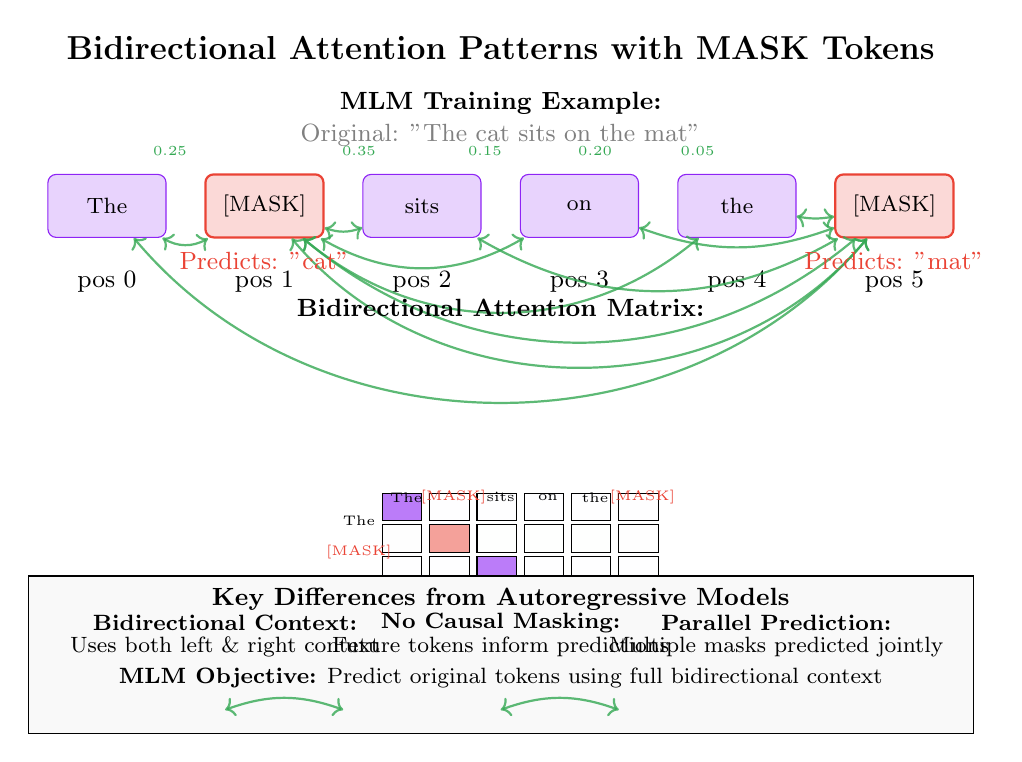
\begin{tikzpicture}[
    token/.style={rectangle, rounded corners=3pt, minimum width=1.5cm, minimum height=0.8cm, font=\footnotesize},
    masktoken/.style={token, fill=maskred!20, draw=maskred, thick},
    normaltoken/.style={token, fill=tokencolor!20, draw=tokencolor},
    attention/.style={<->, thick, attentioncolor, opacity=0.8},
    prediction/.style={->, very thick, maskred},
    label/.style={font=\small},
    title/.style={font=\large\bfseries}
]

% Title
\node[title] at (6, 8.5) {Bidirectional Attention Patterns with MASK Tokens};

% Input sequence with MASK
\node[label] at (6, 7.8) {\textbf{MLM Training Example:}};

% Original text
\node[label, gray] at (6, 7.4) {Original: "The cat sits on the mat"};

% Masked sequence
\node[normaltoken] (t1) at (1, 6.5) {The};
\node[masktoken] (mask1) at (3, 6.5) {[MASK]};
\node[normaltoken] (t3) at (5, 6.5) {sits};
\node[normaltoken] (t4) at (7, 6.5) {on};
\node[normaltoken] (t5) at (9, 6.5) {the};
\node[masktoken] (mask2) at (11, 6.5) {[MASK]};

% Position labels
\node[label, below=0.3cm of t1] {pos 0};
\node[label, below=0.3cm of mask1] {pos 1};
\node[label, below=0.3cm of t3] {pos 2};
\node[label, below=0.3cm of t4] {pos 3};
\node[label, below=0.3cm of t5] {pos 4};
\node[label, below=0.3cm of mask2] {pos 5};

% Bidirectional attention from first MASK
\draw[attention] (mask1) to[bend left=30] (t1);
\draw[attention] (mask1) to[bend right=20] (t3);
\draw[attention] (mask1) to[bend right=30] (t4);
\draw[attention] (mask1) to[bend right=40] (t5);
\draw[attention] (mask1) to[bend right=50] (mask2);

% Bidirectional attention from second MASK
\draw[attention] (mask2) to[bend left=50] (t1);
\draw[attention] (mask2) to[bend left=40] (mask1);
\draw[attention] (mask2) to[bend left=30] (t3);
\draw[attention] (mask2) to[bend left=20] (t4);
\draw[attention] (mask2) to[bend left=10] (t5);

% Attention weights for first MASK
\node[label, attentioncolor, font=\tiny] at (1.8, 7.2) {0.25};
\node[label, attentioncolor, font=\tiny] at (4.2, 7.2) {0.35};
\node[label, attentioncolor, font=\tiny] at (5.8, 7.2) {0.15};
\node[label, attentioncolor, font=\tiny] at (7.2, 7.2) {0.20};
\node[label, attentioncolor, font=\tiny] at (8.5, 7.2) {0.05};

% Predictions
\node[label, maskred] at (3, 5.8) {Predicts: "cat"};
\node[label, maskred] at (11, 5.8) {Predicts: "mat"};

% Attention matrix visualization
\node[label] at (6, 5.2) {\textbf{Bidirectional Attention Matrix:}};

\begin{scope}[shift={(6,2.5)}]
% Create 6x6 attention matrix
\foreach \i in {0,...,5} {
    \foreach \j in {0,...,5} {
        % Different patterns for MASK positions (1 and 5)
        \ifnum\i=1 % First MASK row
            \ifnum\j=1
                \fill[maskred!50] (\j*0.6-1.5, -\i*0.4) rectangle ++(0.5, 0.35);
            \else
                \pgfmathsetmacro{\weight}{0.6 + 0.1*cos(60*\j)}
                \fill[attentioncolor!\weight!white] (\j*0.6-1.5, -\i*0.4) rectangle ++(0.5, 0.35);
            \fi
        \else
            \ifnum\i=5 % Second MASK row
                \ifnum\j=5
                    \fill[maskred!50] (\j*0.6-1.5, -\i*0.4) rectangle ++(0.5, 0.35);
                \else
                    \pgfmathsetmacro{\weight}{0.5 + 0.15*cos(45*\j)}
                    \fill[attentioncolor!\weight!white] (\j*0.6-1.5, -\i*0.4) rectangle ++(0.5, 0.35);
                \fi
            \else % Normal token rows
                \ifnum\j=\i
                    \fill[tokencolor!60] (\j*0.6-1.5, -\i*0.4) rectangle ++(0.5, 0.35);
                \else
                    \pgfmathsetmacro{\weight}{0.3 + 0.1*cos(30*(\i+\j))}
                    \fill[blue!\weight!white] (\j*0.6-1.5, -\i*0.4) rectangle ++(0.5, 0.35);
                \fi
            \fi
        \fi
        \draw[thin] (\j*0.6-1.5, -\i*0.4) rectangle ++(0.5, 0.35);
    }
}

% Matrix labels
\node[label, font=\tiny] at (-1.8, 0) {The};
\node[label, font=\tiny, maskred] at (-1.8, -0.4) {[MASK]};
\node[label, font=\tiny] at (-1.8, -0.8) {sits};
\node[label, font=\tiny] at (-1.8, -1.2) {on};
\node[label, font=\tiny] at (-1.8, -1.6) {the};
\node[label, font=\tiny, maskred] at (-1.8, -2.0) {[MASK]};

\node[label, font=\tiny] at (-1.2, 0.3) {The};
\node[label, font=\tiny, maskred] at (-0.6, 0.3) {[MASK]};
\node[label, font=\tiny] at (0, 0.3) {sits};
\node[label, font=\tiny] at (0.6, 0.3) {on};
\node[label, font=\tiny] at (1.2, 0.3) {the};
\node[label, font=\tiny, maskred] at (1.8, 0.3) {[MASK]};
\end{scope}

% Key insights
\node[rectangle, draw=black, fill=gray!5, minimum width=12cm, minimum height=2cm] at (6, 0.8) {};
\node[label, font=\small\bfseries] at (6, 1.5) {Key Differences from Autoregressive Models};

% Bidirectional flow
\node[label, font=\footnotesize] at (2.5, 1.2) {\textbf{Bidirectional Context:}};
\node[label, font=\footnotesize] at (2.5, 0.9) {Uses both left \& right context};

% No causal masking
\node[label, font=\footnotesize] at (6, 1.2) {\textbf{No Causal Masking:}};
\node[label, font=\footnotesize] at (6, 0.9) {Future tokens inform predictions};

% Multiple predictions
\node[label, font=\footnotesize] at (9.5, 1.2) {\textbf{Parallel Prediction:}};
\node[label, font=\footnotesize] at (9.5, 0.9) {Multiple masks predicted jointly};

% MLM objective
\node[label, font=\footnotesize, align=center] at (6, 0.5) {\textbf{MLM Objective:} Predict original tokens using full bidirectional context};

% Attention flow arrows
\draw[attention, bend left=20] (2.5, 0.1) to (4, 0.1);
\draw[attention, bend right=20] (7.5, 0.1) to (6, 0.1);

\end{tikzpicture}
\end{document}
\caption{Bidirectional attention patterns with \mask{} tokens. The masked position (shown in red) attends to both preceding and following context to make predictions.}
\label{fig:mask_attention}
\end{figure}

Research has shown that models develop sophisticated attention strategies around \mask{} tokens:

\begin{itemize}
\item \textbf{Local Dependencies}: Strong attention to immediately adjacent tokens
\item \textbf{Syntactic Relations}: Attention to syntactically related words (subject-verb, modifier-noun)
\item \textbf{Semantic Associations}: Attention to semantically related concepts across longer distances
\item \textbf{Positional Biases}: Systematic attention patterns based on relative positions
\end{itemize}

\subsubsection{Information Integration Mechanisms}

The model must integrate bidirectional information to make accurate predictions at masked positions. This integration occurs through multiple attention layers that progressively refine the representation:

\begin{align}
h_{\text{mask}}^{(l)} &= \text{Attention}^{(l)}(h_{\text{mask}}^{(l-1)}, \{h_i^{(l-1)}\}_{i \neq \text{mask}}) \\
p(\text{token} | \text{context}) &= \text{Softmax}(W_{\text{out}} \cdot h_{\text{mask}}^{(L)})
\end{align}

where $h_{\text{mask}}^{(l)}$ represents the mask token's hidden state at layer $l$, and the attention mechanism integrates information from all other positions.

\subsection{Advanced Masking Strategies}

Beyond the standard random masking approach, researchers have developed numerous sophisticated masking strategies to improve learning effectiveness.

\subsubsection{Span Masking}

Instead of masking individual tokens, span masking removes contiguous sequences of tokens, encouraging the model to understand longer-range dependencies:

\begin{lstlisting}[language=Python, caption=Span masking implementation]
def create_span_mask(tokens, tokenizer, span_length_distribution=[1,2,3,4,5], 
                     mask_prob=0.15):
    """Create spans of masked tokens"""
    tokens = tokens.copy()
    labels = [-100] * len(tokens)
    
    remaining_budget = int(len(tokens) * mask_prob)
    position = 0
    
    while remaining_budget > 0 and position < len(tokens):
        # Sample span length
        span_length = random.choice(span_length_distribution)
        span_length = min(span_length, remaining_budget, len(tokens) - position)
        
        # Mask the span
        for i in range(position, position + span_length):
            labels[i] = tokens[i]
            tokens[i] = tokenizer.mask_token_id
        
        position += span_length + random.randint(1, 5)  # Gap between spans
        remaining_budget -= span_length
    
    return tokens, labels
\end{lstlisting}

\subsubsection{Syntactic Masking}

Syntactic masking targets specific grammatical elements to encourage learning of linguistic structures:

\begin{lstlisting}[language=Python, caption=Syntactic masking based on POS tags]
def syntactic_mask(tokens, pos_tags, tokenizer, 
                   target_pos=['NOUN', 'VERB', 'ADJ'], mask_prob=0.15):
    """Mask tokens based on part-of-speech tags"""
    tokens = tokens.copy()
    labels = [-100] * len(tokens)
    
    # Find candidates with target POS tags
    candidates = [i for i, pos in enumerate(pos_tags) if pos in target_pos]
    
    # Select subset to mask
    num_to_mask = min(int(len(tokens) * mask_prob), len(candidates))
    mask_positions = random.sample(candidates, num_to_mask)
    
    for pos in mask_positions:
        labels[pos] = tokens[pos]
        tokens[pos] = tokenizer.mask_token_id
    
    return tokens, labels
\end{lstlisting}

\subsubsection{Semantic Masking}

Semantic masking focuses on content words and named entities to encourage learning of semantic relationships:

\begin{example}[Semantic Masking Example]
Original: "Albert Einstein developed the theory of relativity"
Masked: "[MASK] Einstein developed the [MASK] of relativity"

This approach forces the model to understand the relationship between "Albert" and "Einstein" as well as the connection between "theory" and "relativity."
\end{example}

\subsection{Domain-Specific Applications}

Different domains require specialized approaches to \mask{} token usage, each presenting unique challenges and opportunities.

\subsubsection{Scientific Text Masking}

Scientific texts contain domain-specific terminology and structured information that benefit from targeted masking strategies:

\begin{lstlisting}[language=Python, caption=Scientific text masking]
def scientific_mask(text, tokenizer, entity_types=['CHEMICAL', 'GENE', 'DISEASE']):
    """Mask scientific entities and technical terms"""
    # Use NER to identify scientific entities
    entities = extract_scientific_entities(text, entity_types)
    
    tokens = tokenizer.encode(text)
    labels = [-100] * len(tokens)
    
    # Prioritize masking identified entities
    for entity_start, entity_end, entity_type in entities:
        if random.random() < 0.6:  # Higher probability for entities
            for i in range(entity_start, entity_end):
                labels[i] = tokens[i]
                tokens[i] = tokenizer.mask_token_id
    
    return tokens, labels
\end{lstlisting}

\subsubsection{Code Masking}

Code presents unique challenges due to its syntactic constraints and semantic dependencies:

\begin{lstlisting}[language=Python, caption=Code-aware masking]
def code_aware_mask(code_tokens, ast_info, tokenizer, mask_prob=0.15):
    """Mask code tokens while respecting syntactic constraints"""
    tokens = code_tokens.copy()
    labels = [-100] * len(tokens)
    
    # Identify maskable positions (avoid syntax-critical tokens)
    maskable_positions = []
    for i, (token, ast_type) in enumerate(zip(tokens, ast_info)):
        if ast_type in ['IDENTIFIER', 'LITERAL', 'COMMENT']:
            maskable_positions.append(i)
    
    # Select positions to mask
    num_to_mask = int(len(maskable_positions) * mask_prob)
    mask_positions = random.sample(maskable_positions, num_to_mask)
    
    for pos in mask_positions:
        labels[pos] = tokens[pos]
        tokens[pos] = tokenizer.mask_token_id
    
    return tokens, labels
\end{lstlisting}

\subsubsection{Multilingual Masking}

Multilingual models require careful consideration of language-specific characteristics:

\begin{lstlisting}[language=Python, caption=Language-aware masking]
def multilingual_mask(text, language, tokenizer, mask_prob=0.15):
    """Apply language-specific masking strategies"""
    
    # Language-specific configurations
    lang_configs = {
        'zh': {'prefer_chars': True, 'span_length': [1, 2]},
        'ar': {'respect_morphology': True, 'span_length': [1, 2, 3]},
        'en': {'standard_strategy': True, 'span_length': [1, 2, 3, 4]}
    }
    
    config = lang_configs.get(language, lang_configs['en'])
    
    if config.get('prefer_chars'):
        return character_level_mask(text, tokenizer, mask_prob)
    elif config.get('respect_morphology'):
        return morphology_aware_mask(text, tokenizer, mask_prob)
    else:
        return standard_mask(text, tokenizer, mask_prob)
\end{lstlisting}

\subsection{Training Dynamics and Optimization}

The \mask{} token presents unique training challenges that require specialized optimization techniques.

\subsubsection{Curriculum Learning with Masking}

Curriculum learning can improve MLM training by gradually increasing masking difficulty:

\begin{lstlisting}[language=Python, caption=Curriculum masking]
class CurriculumMasking:
    def __init__(self, initial_prob=0.05, final_prob=0.15, warmup_steps=10000):
        self.initial_prob = initial_prob
        self.final_prob = final_prob
        self.warmup_steps = warmup_steps
        self.current_step = 0
    
    def get_mask_prob(self):
        if self.current_step < self.warmup_steps:
            # Linear increase from initial to final probability
            progress = self.current_step / self.warmup_steps
            return self.initial_prob + (self.final_prob - self.initial_prob) * progress
        else:
            return self.final_prob
    
    def step(self):
        self.current_step += 1
\end{lstlisting}

\subsubsection{Dynamic Masking}

Dynamic masking generates different masked versions of the same text across training epochs:

\begin{lstlisting}[language=Python, caption=Dynamic masking implementation]
class DynamicMaskingDataset:
    def __init__(self, texts, tokenizer, mask_prob=0.15):
        self.texts = texts
        self.tokenizer = tokenizer
        self.mask_prob = mask_prob
    
    def __getitem__(self, idx):
        text = self.texts[idx]
        tokens = self.tokenizer.encode(text)
        
        # Generate new mask pattern each time
        masked_tokens, labels = create_mlm_sample(
            tokens, self.tokenizer, self.mask_prob
        )
        
        return {
            'input_ids': masked_tokens,
            'labels': labels
        }
\end{lstlisting}

\subsection{Evaluation and Analysis}

Evaluating \mask{} token effectiveness requires specialized metrics and analysis techniques.

\subsubsection{MLM Evaluation Metrics}

Key metrics for assessing MLM performance include:

\begin{enumerate}
\item \textbf{Masked Token Accuracy}: Percentage of correctly predicted masked tokens
\item \textbf{Top-k Accuracy}: Whether correct token appears in top-k predictions
\item \textbf{Perplexity on Masked Positions}: Language modeling quality at masked positions
\item \textbf{Semantic Similarity}: Similarity between predicted and actual tokens
\end{enumerate}

\begin{lstlisting}[language=Python, caption=MLM evaluation metrics]
def evaluate_mlm(model, test_data, tokenizer):
    """Comprehensive MLM evaluation"""
    total_masked = 0
    correct_predictions = 0
    top5_correct = 0
    semantic_similarities = []
    
    model.eval()
    with torch.no_grad():
        for batch in test_data:
            input_ids = batch['input_ids']
            labels = batch['labels']
            
            outputs = model(input_ids)
            predictions = outputs.logits.argmax(dim=-1)
            top5_predictions = outputs.logits.topk(5, dim=-1).indices
            
            # Evaluate only masked positions
            mask = (labels != -100)
            total_masked += mask.sum().item()
            
            # Accuracy metrics
            correct_predictions += (predictions[mask] == labels[mask]).sum().item()
            
            # Top-5 accuracy
            for i, label in enumerate(labels[mask]):
                if label in top5_predictions[mask][i]:
                    top5_correct += 1
            
            # Semantic similarity (requires embedding comparison)
            pred_embeddings = model.get_input_embeddings()(predictions[mask])
            true_embeddings = model.get_input_embeddings()(labels[mask])
            similarities = F.cosine_similarity(pred_embeddings, true_embeddings)
            semantic_similarities.extend(similarities.cpu().numpy())
    
    metrics = {
        'accuracy': correct_predictions / total_masked,
        'top5_accuracy': top5_correct / total_masked,
        'avg_semantic_similarity': np.mean(semantic_similarities)
    }
    
    return metrics
\end{lstlisting}

\subsubsection{Attention Analysis for \mask{} Tokens}

Understanding how models attend to context when predicting \mask{} tokens provides insights into learned representations:

\begin{lstlisting}[language=Python, caption=Mask token attention analysis]
def analyze_mask_attention(model, tokenizer, text_with_masks):
    """Analyze attention patterns for MASK tokens"""
    input_ids = tokenizer.encode(text_with_masks)
    mask_positions = [i for i, token_id in enumerate(input_ids) 
                     if token_id == tokenizer.mask_token_id]
    
    # Get attention weights
    with torch.no_grad():
        outputs = model(torch.tensor([input_ids]), output_attentions=True)
        attentions = outputs.attentions  # [layer, head, seq_len, seq_len]
    
    # Analyze attention from MASK positions
    mask_attention_patterns = {}
    for mask_pos in mask_positions:
        layer_patterns = []
        for layer_idx, layer_attn in enumerate(attentions):
            # Average over heads
            avg_attention = layer_attn[0, :, mask_pos, :].mean(dim=0)
            layer_patterns.append(avg_attention.cpu().numpy())
        
        mask_attention_patterns[mask_pos] = layer_patterns
    
    return mask_attention_patterns
\end{lstlisting}

\subsection{Best Practices and Guidelines}

Effective \mask{} token usage requires adherence to several established best practices:

\begin{enumerate}
\item \textbf{Appropriate Masking Ratio}: Use 15\% masking as a starting point, adjust based on domain
\item \textbf{Balanced Masking Strategy}: Maintain 80\%/10\%/10\% distribution for robustness
\item \textbf{Dynamic Masking}: Generate new mask patterns across epochs for better generalization
\item \textbf{Domain Adaptation}: Adapt masking strategies to domain-specific characteristics
\item \textbf{Curriculum Learning}: Consider gradual increase in masking difficulty
\item \textbf{Evaluation Diversity}: Use multiple metrics to assess MLM effectiveness
\end{enumerate}

\subsection{Advanced Applications and Extensions}

The \mask{} token has inspired numerous extensions and advanced applications beyond standard MLM.

\subsubsection{Conditional Masking}

Models can learn to condition masking decisions on external factors:

\begin{align}
p(\text{mask}_i | x_i, c) &= \sigma(W_{\text{gate}} \cdot [x_i; c])
\end{align}

where $c$ represents conditioning information such as task requirements or difficulty levels.

\subsubsection{Hierarchical Masking}

Complex documents benefit from hierarchical masking at multiple granularities:

\begin{itemize}
\item \textbf{Token Level}: Standard word/subword masking
\item \textbf{Phrase Level}: Masking meaningful phrases
\item \textbf{Sentence Level}: Masking complete sentences
\item \textbf{Paragraph Level}: Masking entire paragraphs
\end{itemize}

\subsubsection{Cross-Modal Masking}

Multimodal models extend masking to other modalities:

\begin{lstlisting}[language=Python, caption=Cross-modal masking example]
def multimodal_mask(text_tokens, image_patches, mask_prob=0.15):
    """Apply masking across text and vision modalities"""
    
    # Text masking
    text_masked, text_labels = create_mlm_sample(text_tokens, tokenizer, mask_prob)
    
    # Image patch masking
    num_patches_to_mask = int(len(image_patches) * mask_prob)
    patch_mask_indices = random.sample(range(len(image_patches)), num_patches_to_mask)
    
    image_masked = image_patches.copy()
    image_labels = [-100] * len(image_patches)
    
    for idx in patch_mask_indices:
        image_labels[idx] = image_patches[idx]
        image_masked[idx] = torch.zeros_like(image_patches[idx])  # Zero out patch
    
    return text_masked, text_labels, image_masked, image_labels
\end{lstlisting}

The \mask{} token represents a fundamental innovation that enabled the bidirectional language understanding revolution in NLP. Its sophisticated learning paradigm, through masked language modeling, has proven essential for developing robust language representations. Understanding the theoretical foundations, implementation strategies, and advanced applications of \mask{} tokens enables practitioners to leverage this powerful mechanism effectively in their transformer models, leading to improved language understanding and generation capabilities across diverse domains and applications.